%%%%%%%%%%%%%%%%%%%%%%%%%%%%%%%%%%%%%%%%%
% Wenneker Article
% LaTeX Template
% Version 2.0 (28/2/17)
%
% This template was downloaded from:
% http://www.LaTeXTemplates.com
%
% Authors:
% Vel (vel@LaTeXTemplates.com)
% Frits Wenneker
%
% License:
% CC BY-NC-SA 3.0 (http://creativecommons.org/licenses/by-nc-sa/3.0/)
%
% Adapted for COMS30007 by Carl Henrik Ek
%
%%%%%%%%%%%%%%%%%%%%%%%%%%%%%%%%%%%%%%%%%

%----------------------------------------------------------------------------------------
%	PACKAGES AND OTHER DOCUMENT CONFIGURATIONS
%----------------------------------------------------------------------------------------

\documentclass[10pt, a4paper, twocolumn]{article} % 10pt font size (11 and 12 also possible), A4 paper (letterpaper for US letter) and two column layout (remove for one column)

%%%%%%%%%%%%%%%%%%%%%%%%%%%%%%%%%%%%%%%%%
% Wenneker Article
% Structure Specification File
% Version 1.0 (28/2/17)
%
% This file originates from:
% http://www.LaTeXTemplates.com
%
% Authors:
% Frits Wenneker
% Vel (vel@LaTeXTemplates.com)
%
% License:
% CC BY-NC-SA 3.0 (http://creativecommons.org/licenses/by-nc-sa/3.0/)
%
% Adapted for COMS30007 by Carl Henrik Ek
%
%%%%%%%%%%%%%%%%%%%%%%%%%%%%%%%%%%%%%%%%%

%----------------------------------------------------------------------------------------
%	PACKAGES AND OTHER DOCUMENT CONFIGURATIONS
%----------------------------------------------------------------------------------------

\usepackage[english]{babel} % English language hyphenation

\usepackage{microtype} % Better typography

\usepackage{amsthm} % Math packages for equations
\usepackage{amsmath}
\usepackage{amssymb}
\usepackage{mathtools}
\usepackage{bm}
\usepackage{xfrac}
\usepackage{resizegather}



\usepackage[svgnames]{xcolor} % Enabling colors by their 'svgnames'

\usepackage[hang, small, labelfont=bf, up, textfont=it]{caption} % Custom captions under/above tables and figures

\usepackage{booktabs} % Horizontal rules in tables

\usepackage{lastpage} % Used to determine the number of pages in the document (for "Page X of Total")

\usepackage{graphicx} % Required for adding images

\usepackage{enumitem} % Required for customising lists
\setlist{noitemsep} % Remove spacing between bullet/numbered list elements

\usepackage{sectsty} % Enables custom section titles
\allsectionsfont{\usefont{OT1}{phv}{b}{n}} % Change the font of all section commands (Helvetica)

%----------------------------------------------------------------------------------------
%	MARGINS AND SPACING
%----------------------------------------------------------------------------------------

\usepackage{geometry} % Required for adjusting page dimensions

\geometry{
	top= 1.5cm, % Top margin
	bottom=1.5cm, % Bottom margin
	left=1.1cm, % Left margin
	right=1.5cm, % Right margin
	%includehead, % Include space for a header
	includefoot, % Include space for a footer
	%showframe, % Uncomment to show how the type block is set on the page
}

\setlength{\columnsep}{6mm} % Column separation width

%----------------------------------------------------------------------------------------
%	FONTS
%----------------------------------------------------------------------------------------

\usepackage[T1]{fontenc} % Output font encoding for international characters
\usepackage[utf8]{inputenc} % Required for inputting international characters

\usepackage{XCharter} % Use the XCharter font

%----------------------------------------------------------------------------------------
%	HEADERS AND FOOTERS
%----------------------------------------------------------------------------------------

\usepackage{fancyhdr} % Needed to define custom headers/footers
\pagestyle{fancy} % Enables the custom headers/footers

\renewcommand{\headrulewidth}{0.0pt} % No header rule
\renewcommand{\footrulewidth}{0.4pt} % Thin footer rule

\renewcommand{\sectionmark}[1]{\markboth{#1}{}} % Removes the section number from the header when \leftmark is used

%\nouppercase\leftmark % Add this to one of the lines below if you want a section title in the header/footer

% Headers
\lhead{} % Left header
\chead{
%\textit{\thetitle}
} % Center header - currently printing the article title
\rhead{} % Right header

% Footers
\lfoot{} % Left footer
\cfoot{} % Center footer
\rfoot{\footnotesize Page \thepage\ of \pageref{LastPage}} % Right footer, "Page 1 of 2"

\fancypagestyle{firstpage}{ % Page style for the first page with the title
	\fancyhf{}
	\renewcommand{\footrulewidth}{0pt} % Suppress footer rule
}

%----------------------------------------------------------------------------------------
%	TITLE SECTION
%----------------------------------------------------------------------------------------

\newcommand{\authorstyle}[1]{{\large\usefont{OT1}{phv}{b}{n}\color{DarkRed}#1}} % Authors style (Helvetica)

\newcommand{\institution}[1]{{\footnotesize\usefont{OT1}{phv}{m}{sl}\color{Black}#1}} % Institutions style (Helvetica)

\usepackage{titling} % Allows custom title configuration

\newcommand{\HorRule}{\color{DarkGoldenrod}\rule{\linewidth}{1pt}} % Defines the gold horizontal rule around the title

\pretitle{
	\vspace{-20pt} % Move the entire title section up
	\HorRule\vspace{10pt} % Horizontal rule before the title
	\fontsize{32}{36}\usefont{OT1}{phv}{b}{n}\selectfont % Helvetica
	\color{DarkRed} % Text colour for the title and author(s)
}

\posttitle{\par\vskip 15pt} % Whitespace under the title

\preauthor{} % Anything that will appear before \author is printed

\postauthor{ % Anything that will appear after \author is printed
	\vspace{10pt} % Space before the rule
	\par\HorRule % Horizontal rule after the title
	\vspace{20pt} % Space after the title section
}

%----------------------------------------------------------------------------------------
%	ABSTRACT
%----------------------------------------------------------------------------------------

\usepackage{lettrine} % Package to accentuate the first letter of the text (lettrine)
\usepackage{fix-cm}	% Fixes the height of the lettrine

\newcommand{\initial}[1]{ % Defines the command and style for the lettrine
	\lettrine[lines=3,findent=4pt,nindent=0pt]{% Lettrine takes up 3 lines, the text to the right of it is indented 4pt and further indenting of lines 2+ is stopped
		\color{DarkGoldenrod}% Lettrine colour
		{#1}% The letter
	}{}%
}

\usepackage{xstring} % Required for string manipulation

\newcommand{\lettrineabstract}[1]{
	\StrLeft{#1}{1}[\firstletter] % Capture the first letter of the abstract for the lettrine
	\initial{\firstletter}\textbf{\StrGobbleLeft{#1}{1}} % Print the abstract with the first letter as a lettrine and the rest in bold
}

%----------------------------------------------------------------------------------------
%	BIBLIOGRAPHY
%----------------------------------------------------------------------------------------

%\usepackage[backend=bibtex,style=authoryear]{biblatex} % Use the bibtex backend with the authoryear citation style (which resembles APA)

%\addbibresource{example} % The filename of the bibliography

%\usepackage[autostyle=true]{csquotes} % Required to generate language-dependent quotes in the bibliography
 % Specifies the document structure and loads requires packages

\DeclareUnicodeCharacter{2212}{-}
\usepackage{lipsum}
\usepackage{tikz}
\usetikzlibrary{bayesnet}
\usepackage{float}

%Importing relevant materials for the Gaussian plot
\usepackage{pgfplots}
\usepackage{amssymb, amsmath}
\usepackage{tikz}
\usepackage{xcolor}
\pgfplotsset{compat=1.7}
\usepackage{pgfplots}
\usepackage{caption}
\usepackage{subfig}


%----------------------------------------------------------------------------------------
%	ARTICLE INFORMATION
%----------------------------------------------------------------------------------------

\title{Models} % The article title

\author{
	\authorstyle{James O'Reilly\textsuperscript{1} and Adam Pluck\textsuperscript{2}} % Authors
	\newline\newline % Space before institutions
	\textsuperscript{1}\institution{35055}\\ % Institution 1
	\textsuperscript{2}\institution{34013} % Institution 2
}


\date{} % Add a date here if you would like one to appear underneath the title block, use \today for the current date, leave empty for no date

%----------------------------------------------------------------------------------------

\begin{document}

\maketitle % Print the title

\thispagestyle{firstpage} % Apply the page style for the first page (no headers and footers)

%----------------------------------------------------------------------------------------
%	ABSTRACT
%----------------------------------------------------------------------------------------


%----------------------------------------------------------------------------------------
%	ARTICLE CONTENTS
%----------------------------------------------------------------------------------------

\section{The Prior}

\begin{enumerate}

\textbf{Question 1}\\
In the real world there are many factors that can affect our observations. In our example, the given data pairs are corrupted by additive noise. We make the assumption that the factors causing this additive noise are independent.
If our model is given by 
   
\begin{equation}
      \mathbf{y_i} = f(\mathbf{x_i}) + \epsilon
\end{equation}
   
Let each of the N factors causing our noise be an independent variable $\epsilon_i$. The noise in our model is comprised of the sum of these independent variables:
   
\begin{equation}
       \epsilon = \epsilon_1 + \epsilon_2 + ... + \epsilon_n
\end{equation}
   
The Central Limit Theorem states that in some situations, when independent random variables are added, their properly normalised sum tends toward a normal distribution. As we have assumed that the independent variables $\epsilon_i$ causing the noise are independent, we can then apply the Central Limit Theorem and assume that the additive noise in our model follows a Gaussian distribution.\\
  
Choosing a spherical co-variance matrix for the likelihood implies we believe each of the dimensions are independent and that each of the these dimensions vary equally. As every off-diagonal entry in our co-variance matrix is $0$, the dimensions are independent. Each of the dimensions vary equally with variance $\lambda$ because the co-variance takes the form $\lambda\mathbf{I}$. In the case that we choose a non-spherical co-variance, we encode our belief that there exists some dependencies between the dimensions or that each of the dimensions do not vary equally.\\
 
\textbf{Question 2}\\
If we do not assume the data points are independent then we have that $y_1$ is dependent on $X$ and $f$. $y_2$ is dependent on $y_1$, $X$ and $f$, $y_3$ is dependent on $y_1$, $y_2$, $X$ and $f$, etc. Using the product rule of probability we have that:

\begin{equation}
p(\mathbf{Y}\mid f,\mathbf{X}) = p(\mathbf{y_1}\mid f, \mathbf{X})\prod_{i = 2}^{N} p\left( \mathbf{y_i} | f, \mathbf{X}, \{\mathbf{y_1}, ...., \mathbf{y_{i-1}}\} \right)
\end{equation}
  
\textbf{Question 3}\\
Assuming that the values $\mathbf{y_i}$ are independent, we have that
  
  \begin{equation}
      p(\left(\mathbf{Y}|\mathbf{X},\mathbf{W}\right ) = \prod_{i = 1}^N p(\mathbf{y_i}|\mathbf{x_i}, \mathbf{W})
  \end{equation}
  
  which can then be written as 
  
  \begin{equation}
   p(\mathbf{Y}|\mathbf{X},\mathbf{W}) = \prod_{i = 1}^N \frac{exp(-\frac{1}{2}(\mathbf{y_i} - \textbf{W}^{T}\mathbf{x_i})^{T}(\sigma^{2}\textbf{I})^{-1}(\mathbf{y_i} - \textbf{W}^{T}\mathbf{x_i}))}{\sqrt{(2\pi)^D \sigma^{2D}}}
  \end{equation}
  
  where D is the dimension of $\mathbf{X}$.\\
  
  %\begin{equation}
  %    p(\left(\mathbf{Y}|\mathbf{X},\mathbf{W}\right ) = N\left(\mathbf{Y}|\mathbf{WX}, %\sigma ^2 I  \right )
  %\end{equation}
  
  \textbf{Question 4}\\
  Usually, in order to calculate the posterior, we must also calculate the evidence.
  
  \begin{equation}
  Posterior = (Likelihood \cdot Prior)/Evidence
  \end{equation}
  
  For a given probability distribution $p(\mathbf{x}|\mathbf{y})$ if we can find a prior $p(\mathbf{y})$ that is conjugate to the likelihood function, then the posterior distribution will have the same form as the prior. Therefore with the conjugate prior we have that
  
  \begin{equation}
  Posterior \propto Likelihood \cdot Prior
  \end{equation}
  
   As a result, it is no longer necessary to calculate the evidence in order to find the posterior. Conjugate priors are useful in this way because they reduce Bayesian updating to modifying the parameters of the prior distribution rather than computing the ugly and potentially intractable integrals in the evidence.\\
  
  \textbf{Question 5}\\
  For a D-dimensional vector $\mathbf{x}$, the multivariate Gaussian distribution takes the form
  \begin{equation}
  N(\mathbf{x}\mid\mathbf{\mu}, \mathbf{\Sigma}) =  \frac{1}{{{(2\pi) }^{D/2} }}\frac{1}{|\Sigma|^{\frac{1}{2}}}e^{-\frac{1}{2}(\mathbf{x} - \mathbf{\mu})^{T}\Sigma ^{-1}(\mathbf{x} - \mathbf{\mu})}
  \end{equation}
  Our prior over $W$ is therefore of the form 
  \begin{equation}
  p(\mathbf{W}) = \frac{1}{{{(2\pi) }^{D/2} }}\frac{1}{|\Sigma|^{\frac{1}{2}}}e^{-\frac{1}{2}(\mathbf{W} - \mathbf{W}_{0})^{T}\Sigma ^{-1}(\mathbf{W} - \mathbf{W}_{0})}
  \end{equation}
  
  From this we can see that the functional dependence of the Gaussian on W is entirely on the exponent. The exponent is in fact the squared Mahalanobis distance given by
  
  \begin{equation}
      D_m(x,\mathbf{x_0},\mathbf{\Sigma}) = \sqrt[]{(x-\mathbf{x_0})^T \mathbf{\Sigma}^{-1} (x-\mathbf{x_0})}
  \end{equation}
  
  However, in the case of a spherical co-variance matrix, the Mahalanobis distance function reduces down to the Euclidean distance scaled by some constant.\\
  
  \textbf{Question 6}\\ 
  From previous questions we know the distributions of both our likelihood and prior.
  
  \begin{align}
    Likelihood &\sim N(\mathbf{Y}|\mathbf{W}\mathbf{X}, \sigma^2\mathbf{I)}\\
    Prior &\sim N(\mathbf{W}_{0}, \tau^2\mathbf{I})\\
    Posterior &\propto Likelihood * Prior
  \end{align}
  

  The self-conjugacy property of a Gaussian means that we can disregard the evidence and calculate the posterior by simply calculating the product of the likelihood and prior. As Gaussian distributions are self-conjugate, we know that the posterior will also be a Gaussian. This means that we just need to inspect the constant, linear and quadratic terms of $\mathbf{W}$ in the exponent of $P(\mathbf{Y}|\mathbf{X},\mathbf{W})P(\mathbf{W})$ to determine the mean and co-variance.
  
   \begin{equation}
      Posterior \propto e^{-\frac{1}{2\sigma^2}(\mathbf{Y}-\mathbf{W}^T\mathbf{X})^T(\mathbf{Y}-\mathbf{W}^T\mathbf{X})}e^{-\frac{1}{2\tau^2}(\mathbf{W}-\mathbf{W_0})^T(\mathbf{W}-\mathbf{W_0})}
  \end{equation}
  
  \begin{equation}
      Constant = exp\{-\frac{1}{2}(\sigma^{-2}\mathbf{Y}^T\mathbf{Y}+\tau^{-2}\mathbf{W_0}^T\mathbf{W_0})\}
  \end{equation}
  
  \begin{equation}
      Linear = exp\{\sigma^{-2}\mathbf{Y}^T\mathbf{W^T}\mathbf{X}+\tau^{-2}\mathbf{W_0^TW}\}
  \end{equation}
  
  \begin{equation}
      Quadratic = exp\{-\frac{1}{2}(\sigma^{-2}\mathbf{({W}^T\mathbf{X})}^T(\mathbf{W}^T\mathbf{X})+\tau^{-2}\mathbf{W}^T\mathbf{W})\}
  \end{equation}
  
  This leaves us with a posterior in the form:
  
  \begin{equation}
      P(\mathbf{W}|\mathbf{X}, \mathbf{Y}) = N(\mathbf{W}| \mathbf{m}_n, \mathbf{S}_n)
  \end{equation}
  
  where:
  
  \begin{equation}
      \mathbf{m}_n = \mathbf{S_n}(\frac{1}{\tau^2}\mathbf{W_0} + \frac{1}{\sigma^2}\mathbf{X}\mathbf{Y})\\
      \mathbf{S}_n = (\frac{1}{\tau^2}+ \frac{1}{\sigma^2}\mathbf{X}\mathbf{X}^T)^{-1}
  \end{equation}
  
  \textbf{Question 7}\\
  Non-parametric models assume that the distribution of the data cannot be defined in terms of a finite set of parameters. In doing so, non-parametric machine learning algorithms don't make strong assumptions about the form of the underlying function. This lack of constraint means that they are free to learn any functional form from the training data.\\
  
  Parametrisation of data:
  With non-parametric methods we have the advantage of not having to assume the algebraic form of the function (the number of parameters isn't fixed). This lack of constraint means that they are free to learn any functional form from the training data, allowing for a more flexible model. Furthermore, as no assumptions are made about the underlying function, the model will become more accurate as we feed it more data. In contrast, parametric machine learning models first assume the underlying function has a fixed number of parameters and then learn the parameters from the training data. No matter how much data you throw at a parametric model, it won't change its mind about how many parameters it needs.\\
  
  Interpretability of models:
  While parametric models are constrained to a fixed form and have limited complexity, they are much easier to interpret and understand. As we have assumed their functional form, we know how many parameters the model has. Furthermore, we can see how the parameters change over time and interpret what this means. Non-parametric models are more difficult to interpret. As we have not assumed the functional form, we know very little about the parameters and how they behave as our model evolves. The key trade-off is between flexibility/complexity and interpretability. What we gain in complexity and flexibility, we lose in interpretability and it is harder to explain why specific predictions are made.\\
  
  \textbf{Question 8}\\
  In Bayesian probability we use priors to encode our beliefs (or assumptions) about the data. With Gaussian processes we define a prior probability distribution over functions directly. A Gaussian process prior therefore represents our belief about the unknown function \textbf{f} via the mean and our co-variance matrix defined by the kernel function \textbf{K}. With the mean and co-variance we encode our beliefs about how the function should behave: whether or not the function is periodic, the smoothness of the function, etc. The co-variance matrix generated by this kernel function outlines how exactly different points co-vary with respect to each other.\\
  
  How does this process place structure on the space of functions? By weighting toward functions that conform to our co-variance matrix, the GP prior effectively limits the properties that our function can have, and therefore places a probabilistic structure on the space of functions. Take smoothness, for example. Our belief is that the function that generates the data is smooth. We wish to encode this prior knowledge with our Gaussian Process and so we specify via our kernel function that we want our function to be smooth. We do this by effectively telling our function approximator that if two points $x_i$ and $x_j$ are close to one another, then their heights $f(x_i)$ and $f(x_j)$ will also be similar. This idea of similarity is represented by the different entries in our co-variance matrix. A large co-variance between $x_i$ and $x_j$ means that $f(x_i)$ and $f(x_j)$ are close to one another. More intuitively, given $f(x_i)$ we can infer more about the value of $f(x_j)$.\\
  
  \textbf{Question 9}\\
  The Gaussian nature of the GP prior ensures that it encodes all possible functions and weights toward the functions that best fit our data. While there are some functions that fit the data terribly, each and every possible function is attributed a probability and is thus encoded by our prior. It is important to note that for a finite training set it is only necessary to consider the values of the function at the discrete set of input variables $\mathbf{x_n}$. We can do this because Kolmogorov's Extension Theorem\cite{Kolmogorov} guarantees that a suitably "consistent" collection of finite-dimensional distributions will define a stochastic process. This means that in practice we can work in a finite space.\\
  
  \textbf{Question 10}\\
  The joint distribution of the full model is given by
  \begin{equation}
      p(\mathbf{Y},\mathbf{X},f,\mathbf{\Theta}) = p(\mathbf{Y}\mid\mathbf{X},f,\mathbf{\Theta})\cdot(p{f\mid\mathbf{X}, \mathbf{\Theta})}\cdot{p(\mathbf{X},\mathbf{\Theta})}
  \end{equation}
  
  The dependencies in this model can be represented by the following graphical model:
  
  \begin{figure}[H]
      \centering
      \begin{tabular}{cc}
        % model_pca.tex
%
% Copyright (C) 2012 Jaakko Luttinen
%
% The MIT License
%
% See LICENSE file for more details.

% PCA model

%\beginpgfgraphicnamed{model-pca}
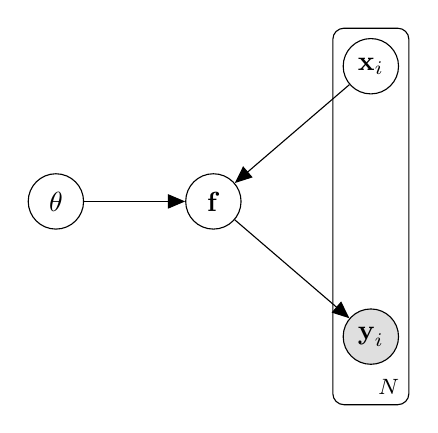
\begin{tikzpicture}

  % Define nodes
  \node[obs]                               (y) {$\textbf{y}_i$};
  \node[latent, above=of y, xshift=-2cm] (f) {$\mathbf{f}$};
  \node[latent, above=of y, xshift=-4cm] (t) {$\theta$};
  \node[latent, above=of f, xshift=2cm]    (x) {$\textbf{x}_i$};

  % Connect the nodes
  \edge {x,t} {f};
  \edge {f} {y};

  % Plates
  \plate {yx} {(x)(y)} {$N$} ;

\end{tikzpicture}
%\endpgfgraphicnamed

%%% Local Variables:
%%% mode: tex-pdf
%%% TeX-master: "example"
%%% End:

      \end{tabular}
      \caption{Graphical model showing the dependencies in our model}
      \label{fig:my_label}
  \end{figure}
  
  \begin{itemize}
      \item We assume zero mean for the Gaussian prior and our assumptions about the nature of the function are encoded by our choice of kernel and the hyper-parameters $\mathbf{\theta}$.
  \end{itemize}
  \begin{itemize}
      \item We have assumed that $\mathbf{Y}$ may not be completely determined by $\mathbf{X}$ and $f$, instead our likelihood function encodes the fact that $\mathbf{Y}$ may be corrupted by Gaussian noise.
  \end{itemize}
  \begin{itemize}
      \item We assume that $\mathbf{X}$ and $\mathbf{\Theta}$ are independent. Based on our assumption that $\mathbf{X}$ and $\mathbf{\Theta}$ are independent we have that (7) can now be reduced to
     \end{itemize}
\begin{equation}
      p(\mathbf{Y},\mathbf{X},f,\mathbf{\Theta}) = p(\mathbf{Y}\mid\mathbf{X},f,\mathbf{\Theta})\cdot(p{f\mid\mathbf{X}, \mathbf{\Theta})}\cdot{p(\mathbf{X})}\cdot{p(\mathbf{\Theta})}
\end{equation}
  
  Annoyingly, we have added a new variable which we are not really interested in. Specifically we have modelled the relationship between $\mathbf{Y}$ and $f$ and also $f$ and $\mathbf{X}$ but what we are really interested in is the relationship between $\mathbf{Y}$ and $\mathbf{X}$. We should therefore marginalise out $f$ which involves computing the integral
  
  \begin{equation} \label{eq:23}
      p(\mathbf{Y}\mid \mathbf{X},\mathbf{\Theta}) = \int p(\mathbf{Y}\mid f)p(f\mid \mathbf{X},\mathbf{\Theta})df 
  \end{equation}
  
  \textbf{Question 11}\\
  How does equation (\ref{eq:23}) connect the prior to the data? The likelihood $p(\mathbf{Y}|f)$ is characterised entirely by the function $f$ given by the prior. The prior $p(f|\mathbf{X},\mathbf{\theta})$ gives a distribution of $f$s given $\mathbf{X}$ and $\mathbf{\theta}$. When we marginalise out $f$ we are feeding the different choices of $f$ into our likelihood $p(\mathbf{Y}|f)$. Therefore when we compute the integral we effectively get the weighted average of this distribution of $f$s. This process directly connects our prior $p(f|\mathbf{X},\mathbf{\theta})$ to our data. 
  
  How does uncertainty 'filter' through the model?
  There are two causes of uncertainty in the model. The first cause of uncertainty is in the choice of $f$. The second cause of uncertainty the additive Gaussian noise $\epsilon$ that is affecting our target variable $Y$.
  
  \begin{equation}
      \mathbf{y_i} = f(\mathbf{x_i}) + \epsilon
  \end{equation}
  
  Note that in (\ref{eq:23}), we have marginalised out $f$, however the uncertainty present in our choice of $f$ still remains. This process of marginalisation can be seen as taking the uncertainty present in our choice of $f$ and feeding into the likelihood. It's important to note that when uncertainty is said to be 'filtered through', this does not mean that the uncertainty is 'filtered out' and is now longer present in the model. Instead, it more so refers to the idea that the uncertainty present in $f$ is being effectively transferred from $f$ to $\mathbf{Y}$ and by the process of marginalising $f$. The resultant distribution is then Gaussian, as both the likelihood and the prior are Gaussian. This concept of uncertainty 'filtering' through fits intuitively with the graphical model above, as after removing $f$, we still have that $\mathbf{Y}$ is dependent on $\mathbf{X}$ and $\mathbf{\theta}$.
  
  The second cause of uncertainty, the additive Gaussian noise affecting our target variable $Y$, remains unaffected by the marginalisation of $f$. As can be seen in the equation (24), $\epsilon$ is completely independent of $f$, $\mathbf{X}$ and $\mathbf{\theta}$.
  
  After marginalisation, the LHS of (8) is given by $p(\mathbf{Y}\mid \mathbf{X},\mathbf{\Theta})$. From this expression we can see that $Y$ is now directly dependent on $\mathbf{\theta}$ as we have marginalised out $f$.\\
      
 \textbf{Question 12}\\
 We assume that the prior $P(\mathbf{W})$ is a zero-mean isotropic Gaussian:  $P(\mathbf{W})\sim N(\mathbf{W}|\mathbf{0},\alpha^{-1}\mathbf{I})$. Setting $\alpha = 1$ we can visualise the prior (see Figure \ref{fig:Q12_Prior_1}).
      
\begin{figure}[]
      \centering
      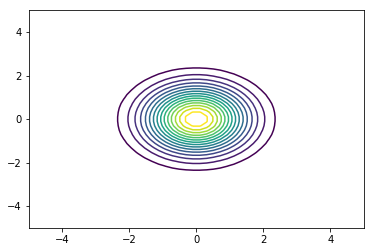
\includegraphics[width = 0.46\textwidth]{imagesfinal/finalpriorQ12.png}
      \caption{Prior distribution over $\mathbf{W}$}
      \label{fig:Q12_Prior_1}
  \end{figure}
      
%The Gaussian Prior is centred at (0,0) as our mean is the zero vector. The horizontal and vertical principle axes show that the dimensions are independent which is specified by the spherical co-variance matrix in the prior.

Training the model with a single data point (-1, 1.50243220) and then sampling from the posterior, we see that the model is generally imprecise with the sampled functions disagreeing wildly (see Figure 3). We also see that the updated posterior distribution has a large co-variance, implying there is still a large degree of uncertainty in the model (see Figure 4).
  
\begin{figure}[]
      \centering
      \captionsetup{justification=centering, margin = 1cm}
      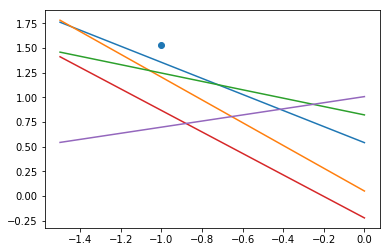
\includegraphics[width = 0.46\textwidth]{imagesfinal/Q12_finalposterior_1_.png}
      \caption{Samples from the posterior after training with one data point}
      \label{fig:Q12_posterior_1}
  \end{figure}
  
\begin{figure}[H]
      \centering
      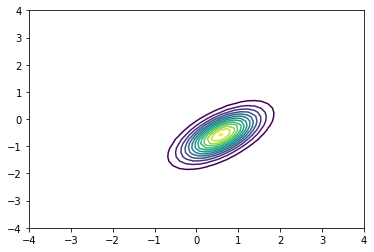
\includegraphics[width = 0.46\textwidth]{imagesfinal/q12_finalposterior_2.png}
      \caption{Updated posterior trained with one data point}
      \label{fig:Q12_sample_1}
  \end{figure}
      
Once the posterior is updated with 50 more data points, we can see that distribution now has a much narrower spread which implies there is less uncertainty in our model (see Figure \ref{fig:Q12_sample_2}). As a result of this, the functions sampled from the posterior fit the data points well (see Figure \ref{fig:Q12_posterior_2}).
      
\begin{figure}[H]
      \centering
      \captionsetup{justification=centering, margin = 1cm}
      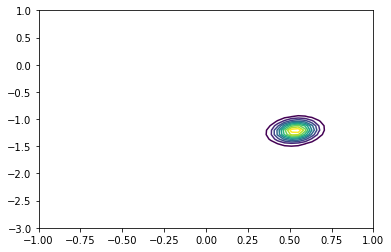
\includegraphics[width = 0.46\textwidth]{imagesfinal/Q12_finalposterior_4.png}
      \caption{Updated posterior trained with 50 data points}
      \label{fig:Q12_sample_2}
  \end{figure}
  
  \begin{figure}[H]
      \centering
      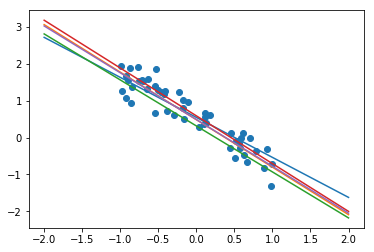
\includegraphics[width = 0.46\textwidth]{imagesfinal/Q12_finalposterior_3.png}
      \caption{Samples from the posterior with 50 data points}
      \label{fig:Q12_posterior_2}
  \end{figure}
      
The accuracy of the model improves dramatically as it is trained with more data points.

Why does the model exhibit this behaviour as we perform the Bayesian updating? We can explain this behaviour by looking at the form of the co-variance of our posterior distribution given in (20). As the number of data points ($\mathbf{X}$) increases, the $\mathbf{XX}^T$ term also increases, thus reducing the overall co-variance of the posterior distribution. If we continued to train the model with larger data-sets, the co-variance of the posterior would continue to decrease, giving a more homogeneous set of samples.\\   

\textbf{Question 13}\\
   Having illustrated the process of learning with a parametric model, we will now investigate a non-parametric model: Gaussian processes. The Gaussian process prior is defined here with mean $\mathbf{0}$ and a squared exponential co-variance function
  
  \begin{equation}
      k(\mathbf{x_i},\mathbf{x_j}) = \sigma^{2}fe^\frac{-(\mathbf{x_i}-\mathbf{x_j})^T(\mathbf{x_i}-\mathbf{x_j})}{l^{2}}
  \end{equation}
  
  Where the $l$ is a hyper-parameter of the Gaussian process called the length-scale. Drawing samples from the GP prior and plotting them, we can see how the nature of our samples change as we alter the length-scale.
  
  \begin{figure}[H]
      \centering
      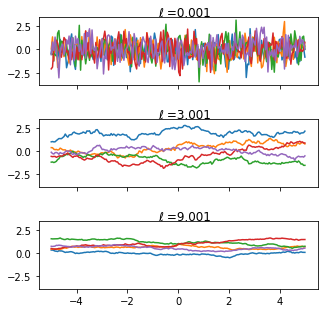
\includegraphics[width = 0.43\textwidth]{images/nonparametricprior.png}
      \caption{}
      \label{fig:Q13_non-parametric_prior}
  \end{figure}
  
  How do we explain this behaviour mathematically? Looking at equation (25), we note that as the value of the length-scale increases, the value of $k(\mathbf{x_i},\mathbf{x_j})$ also increases, meaning that $f(\mathbf{x_i})$ and $f(\mathbf{x_j})$ now co-vary more together. By increasing the length-scale, we ensure that values that are close together in input space will produce output values that are close together, giving a smoother function.
  
  The length-scale encodes our assumption about the smoothness of the function. This assumption is based on our belief that functions in the real world tend to be smooth. More, specifically the length-scale encode our assumption about the degree at which the distance between $\mathbf{x_i}$ and $\mathbf{x_j}$ determines the certainty of $f(\mathbf{x_j})$ given $f(\mathbf{x_i})$.
   
  How exactly does the length-scale encode this relationship between $\mathbf{x_i}$, $\mathbf{x_j}$, $f(\mathbf{x_i})$, $f(\mathbf{x_j})$? A useful way to generate intuition for this concept is to view the univariate normal distribution of $f(\mathbf{x_j})$ given $f(\mathbf{x_i})$:
   
\begin{equation}
    p(f(x_j)\mid f(x_j))\sim \mathcal{N}(f(x_i), \tau^{2})
\end{equation}

   It is instructive to view how this conditional distribution changes as we alter the length-scale. 
   
   %insert plot of 3 univariate normals
   \pgfmathdeclarefunction{gauss}{2}{%
  \pgfmathparse{1/(#2*sqrt(2*pi))*exp(-((x-#1)^2)/(2*#2^2))}%
}
\begin{tikzpicture}
\begin{axis}[
  no markers, domain=-15:15, samples=100,
  axis lines*=left, xlabel=$x$, ylabel=$y$,
  every axis y label/.style={at=(current axis.above origin),anchor=south},
  every axis x label/.style={at=(current axis.right of origin),anchor=west},
  height=5cm, width=8.5cm, legend entries={$l=5$,$l=2$,$l=1$},
  xtick={-12,-8,-4,0,4,8,12}, ytick=\empty,
  enlargelimits=false, clip=false, axis on top,
  grid = major
  ];
  \addplot [very thick,cyan!50!black] {gauss(0,0.85)};
  \addplot [very thick,red!50!black] {gauss(0,2)};
  \addplot [very thick,black!50!black] {gauss(0,5)};

%\draw [yshift=-0.6cm, latex-latex](axis cs:4,0) -- node [fill=white] {} (axis cs:5.96,0);
\end{axis}
\end{tikzpicture}
   
   We can see that as the value of our length-scale increases, the variance of $p(f(x_j)\mid f(x_i))$ decreases, implying that we are more certain about the position of $f(x_j)$ about the mean $f(x_i)$. The relationship between the variance of the conditional $\tau^2$ and the length-scale $l$ can be modelled by
   
   \begin{equation}
       \tau^2 \propto \frac{1}{l}
   \end{equation}
   
   As the value of the length-scale increases, the variance of our conditional distribution decreases which yields a smoother function.\\

  \textbf{Question 14}\\
  The prior defined previously can now be used to compute the predictive posterior distribution. We introduce the data generated by an unknown function $f$ and then draw samples. When compared with samples from our prior, we can see that as the model has been trained with some data, samples taken from the posterior better fit the underlying function.
  
  In the first sample there is complete certainty in the $Y$ values as we have assumed a noiseless model. This is illustrated by the fact that each sample passes through each of the data points. Having only a small number of data points on which to train the model, it is unrealistic to assume these points will fully represent the function from which they were generated. This increases the risk of over-fitting.
  
  \begin{figure}[H]
      \centering
      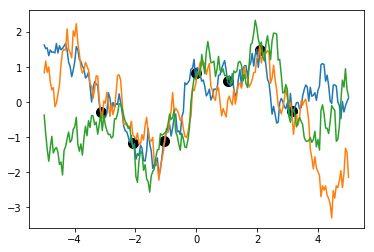
\includegraphics[width=70mm, scale=0.5]{imagesfinal/Q14_sample_no_error.png}
      \label{fig:Q14_Posterior_no_error}
      \caption{Three samples from the posterior \textbf{without error}}
  \end{figure}
  
  To mitigate this risk we add a spherical co-variance matrix $\lambda I$ to our kernel function. This $\lambda$ should be the same value as the variance of the Gaussian noise generated in our model. This gives a function that doesn't fit the data exactly but gives a more honest representation of the underlying function that generated our data.
   
 \begin{figure}[H]
      \centering
      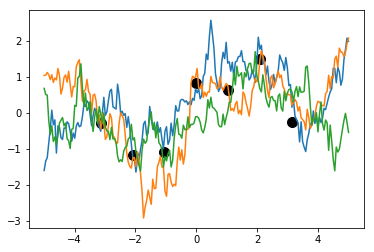
\includegraphics[width=70mm, scale=0.5]{imagesfinal/Q14_sample_error.png}
      \label{fig:Q14_Posterior_error}
      \caption{Three samples from the posterior \textbf{with error}}
  \end{figure}
 
Plotting the data, predictive mean, and predictive variance with $\sigma = 1$, we can see that our variance decreases around the training data as we are more certain about the $y$ values and the variance increases away from the data points (see Figure 10). The absence of data reduces the constraint put on the function. Note that even at the data points, there is still uncertainty as we have factored Gaussian noise into the model.
 
 \begin{figure}[H]
      \centering
      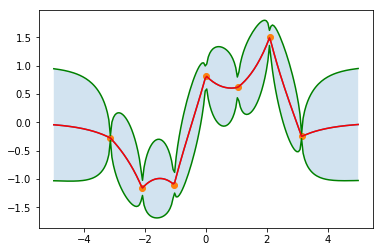
\includegraphics[width=70mm, scale=0.5]{imagesfinal/Q14_predictive_variance.png}
      \label{fig:Q14_Predictive}
      \caption{}
  \end{figure}

\section{Posterior}

  \textbf{Question 15}\\
  Belief: "An acceptance that something exists or is true, especially one without proof."[Oxford]\newline
  Assumption: "A thing that is accepted as true or as certain to happen, without proof."[Oxford]\newline
  
  Based purely on the their definitions, beliefs and assumptions seem equivalent and interchangeable. If the two concepts are truly equivalent, then there is little to say about how they relate to each other. We need not accept this equivalence, however. Perhaps beliefs and assumptions are distinct and we can view them as mutually dependent rather than equivalent? When we believe, we hold a certain proposition to be true (as given by the definition above). In doing so, one makes the \textit{a priori} assumption in the veracity of that belief and so beliefs require this \textit {a priori} assumption to even get off the ground.
  
  Crucially, note that the \textit{a priori} assumption the belief relies upon is provisional. This means that there are two outcomes:
  \begin{enumerate}
      \item The assumption will be ratified at some point in the future, when there is convincing evidence to confirm or refute the assumption, making it true or false.
      \item The assumption will not be ratified.
  \end{enumerate}
  If the assumption is ratified, then we can conclude whether or not our belief is true, as the foundation on which it is built will be shown to be stable or unstable. If, on the other hand, the assumption is not ratified, then no conclusions can be made as to the veracity of the belief. We must therefore accept that all beliefs are provisional because they are buttressed by provisional assumptions.
  
  How do preferences relate to both assumptions and beliefs? The idea of preference implies an ordering of some sort. Before any set can be ordered, each element must have some well-defined property which can be compared. Therefore, before a preference is specified, there must exist a belief about each of the elements. In this regard, preference can be viewed as the process of imposing a hierarchy on a set of beliefs.
  
  How does this apply within the context of machine learning models?  When we train machine learning models, we already have beliefs about the world. These beliefs are encoded in our assumptions about models that describe the world. More specifically, we use prior distributions as a means of encoding our beliefs about data before we begin to learn. What do we mean by preference in this context? As mentioned above, preferences can be viewed as placing a hierarchy on a set of beliefs or assumptions. For example, we may prefer to represent our data with a linear model, and so we encode that preference in our assumptions that the model is of the form $\mathbf{y_i} = f(\mathbf{x_i}) + \epsilon$. In this regard our preferences also inform the assumptions we make.\\
  
  \textbf{Question 16}\\
  By specifying the prior over $\mathbf{X}$ to be a spherical Gaussian, we are assuming that each of the dimensions are independent and have equal variance. This assumption isn't justified by any data, it is merely a preference. Why is it preferable for our prior to be have this distribution? Gaussian distributions are self-conjugate, and so setting our prior $p(\mathbf{X})$ to be Gaussian saves us from calculating the evidence when we perform Bayesian updating. Why specifically spherical instead of Gaussian? Performing Gaussian convolution when marginalising is much simpler with a simple Gaussian we have chosen. Again, this is just a preference we have rather than a belief that is motivated by any specific observation.
  
  \textbf{Question 17}\\
  From the conditional probability we have that:
  \begin{equation}
     P(\mathbf{Y}, \mathbf{X}, \mathbf{W}) = P(\mathbf{Y}|\mathbf{X}, \mathbf{W})P(\mathbf{X})P(\mathbf{W})
  \end{equation}
  We then marginalise out $X$
  
  \begin{align}
    P(\mathbf{Y},\mathbf{W}) &= \int_{}^{} P(\mathbf{Y}, \mathbf{X}, \mathbf{W})  d\mathbf{X}\\
    &=  \int_{}^{} P(\mathbf{Y}|\mathbf{X}, \mathbf{W})P(\mathbf{X})P(\mathbf{W}) d\mathbf{X}\\
    &= P(\mathbf{W}) \int_{}^{} P(\mathbf{Y}|\mathbf{X}, \mathbf{W})P(\mathbf{X}) d\mathbf{X}\\
    &= P(\mathbf{W}) P(\mathbf{Y}|\mathbf{W})
  \end{align}
 
    (n.b in Eq (30) we know that $P(\mathbf{W})$ is independent of $\mathbf{X}$ so we can factor it out of the integral)\\

\textbf{Question 18}
 \begin{enumerate}
 
\item 
Maximum \textit{a posteriori} estimation takes into account prior beliefs as well as the likelihood and tries to maximise the posterior. In contrast, Maximum Likelihood is concerned exclusively with the likelihood function and isn't concerned with priors.
Maximum likelihood estimation finds the parameters that maximise the likelihood function. It is essentially a special case of MAP estimation with a uniform prior probability.
Type 2 Maximum Likelihood estimation tries to find parameters that maximise the marginal likelihood.\\

\item      
Note that as we observe more data MAP and ML will converge to the same value(s) because the effect the prior has on the likelihood becomes less significant as we add more data. \\
      
\item
In the optimisation problem given by equation (33) we are able negate the integral denominator and just optimise over the numerator. This is possible as the denominator is both positive (as all proper probabilities are) and independent of $\mathbf{W}$ (as it is the marginalisation on $\mathbf{W}$) . For these reasons it plays no role in the maximisation and the optimisation problem is reduced to maximising $\mathbf{W}$ in equation (34).     

\begin{equation}
    \text{argmax}_\mathbf{W}\frac{P(\mathbf{Y}|\mathbf{X},\mathbf{W})P(\mathbf{W})}{\int_{}^{} P(\mathbf{Y}|\mathbf{X},\mathbf{W})P(\mathbf{W})d\mathbf{W}}\\
    = \text{argmax}_\mathbf{W}P(\mathbf{Y}|\mathbf{X},\mathbf{W})P(\mathbf{W})
\end{equation}
    
    
\end{enumerate}
   
\textbf{Question 19}\\
  We can assume that the posterior has a co-variance as some function $\mathbf{C}$
  where $\mathbf{C} = \mathbf{W}\mathbf{W}^T + \sigma^2\mathbf{I}$ and $\sigma^2$ is the variance of the noise. Following this we can derive a log-likelihood function as follows:
  
  \begin{equation}
    L(\mathbf{W}) = c + \frac{N}{2}\ln{|\mathbf{C}|} +  \frac{1}{2}\sum_{i=1}^{N} y_i^T\mathbf{C}^{-1}y_i
  \end{equation}
  
  We can then rewrite this and calculate the derivatives:
  
  \begin{equation}
      L(\mathbf{W}) = c + \frac{1}{2}\ln{|\mathbf{C}|} +  \frac{1}{2}tr(\mathbf{Y}\mathbf{C}^{-1}\mathbf{Y}^T)
  \end{equation}
  
  \begin{equation}
      \frac{\partial L(\mathbf{W})}{\partial W_{ij}} = tr(\mathbf{C^{-1}}\frac{\partial \mathbf{C}}{\partial W_{ij}}) 
    + tr(\mathbf{Y}\mathbf{Y}^T(-\mathbf{C^{-1}} \frac{ \partial \mathbf{C}}{\partial W_{ij}} \mathbf{C^{-1}})
  \end{equation}
  
  \begin{equation}
     \frac{\partial L(\mathbf{W})}{\partial W_{ij}} = tr(\mathbf{C^{-1}}\frac{\partial \mathbf{W}\mathbf{W}^T}{\partial W_{ij}}) + tr(\mathbf{Y}\mathbf{Y}^T(-\mathbf{C^{-1}} \frac{ \partial \mathbf{\mathbf{W}\mathbf{W}^T}}{\partial W_{ij}} \mathbf{C^{-1}})
    \end{equation}
  
  \textbf{Question 20}\\
  Marginalising out $\mathbf{X}$ is troublesome for two main reasons. First, suppose we have a directed chain of dependency between $n$ random variables with each random variable able to take on $z$ different values:
  
  \begin{figure}[H]
      \centering
      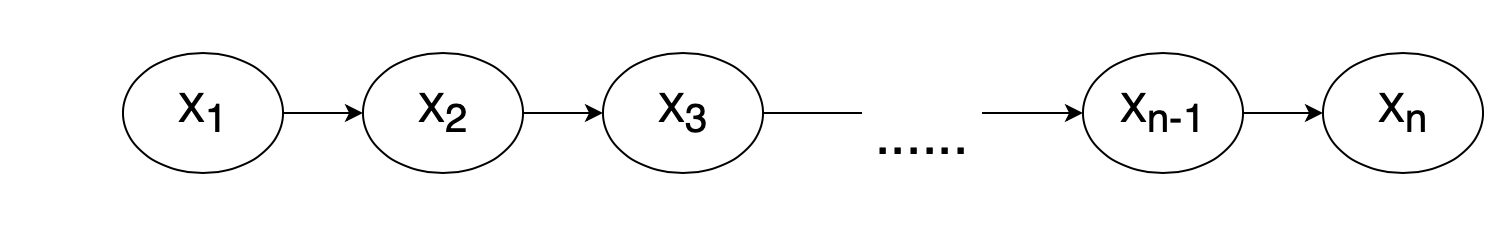
\includegraphics[width=75mm,scale=0.5]{images/q20.png}
      \label{fig:Q20_graph_1}
  \end{figure}
 
  If we want to calculate 
  \begin{equation} 
    P(X_{n} = x) = \sum_{X_{1}...X_{n}}^{} P(X_{1}X_{2}...X_{n-1}X_{n}) 
  \end{equation}
  
  We have to marginalise over all variables $\{{X_{1}...X_{n-1}\}}$ requiring $O(z^n)$ computations. When we have large sets of variables, this calculation quickly becomes computationally expensive.
  
   We can therefore define a general function $f$ such that
   \begin{equation}
    f: \left(\{{X_{1}...X_{n-1}\}} , \theta \right)       \xrightarrow{} Y
   \end{equation}
   
   Y now depends on $f$ and $f$ depends on $\{X_{n}\}$ and $\theta$. This means we can just marginalise over f whilst still utilising the information provided by ${X_n}$ and $\theta$.\\
   
   Secondly, when marginalising in the past, we have been able to repeatedly perform Gaussian convolutions as it was assumed that the variable we were marginalising over was distributed $N(\mu,\mathbf{C})$ where $\mathbf{C}$ is a linear function of the variable we are marginalising on.\\
   
   In the real world, however, it is unlikely that our variable(s) would be distributed so conveniently. In the case that the random variable we are marginalising over is given by $N(\mu, k(x))$ where $k(x)$ is a non-linear function of $x$, each Gaussian convolution yields a more complex co-variance in the resultant product and as a result the marginalisation is analytically intractable.\\
   
   Marginalising over $f$ solves both of these problems. As $f$ is closer to $Y$ in the chain of dependencies, performing the marginalisation is less expensive computationally. Furthermore, we can define $f$ to guarantee the co-variance of the Gaussian is not a non-linear function and so our marginalisation involves simple Gaussian convolutions.\\    

  \textbf{Question 21}
  
  In Figure 11 we can clearly see a spiral with the points increasing in spread as we come further out of the spiral:
  
  \begin{figure}[H]
      \centering
      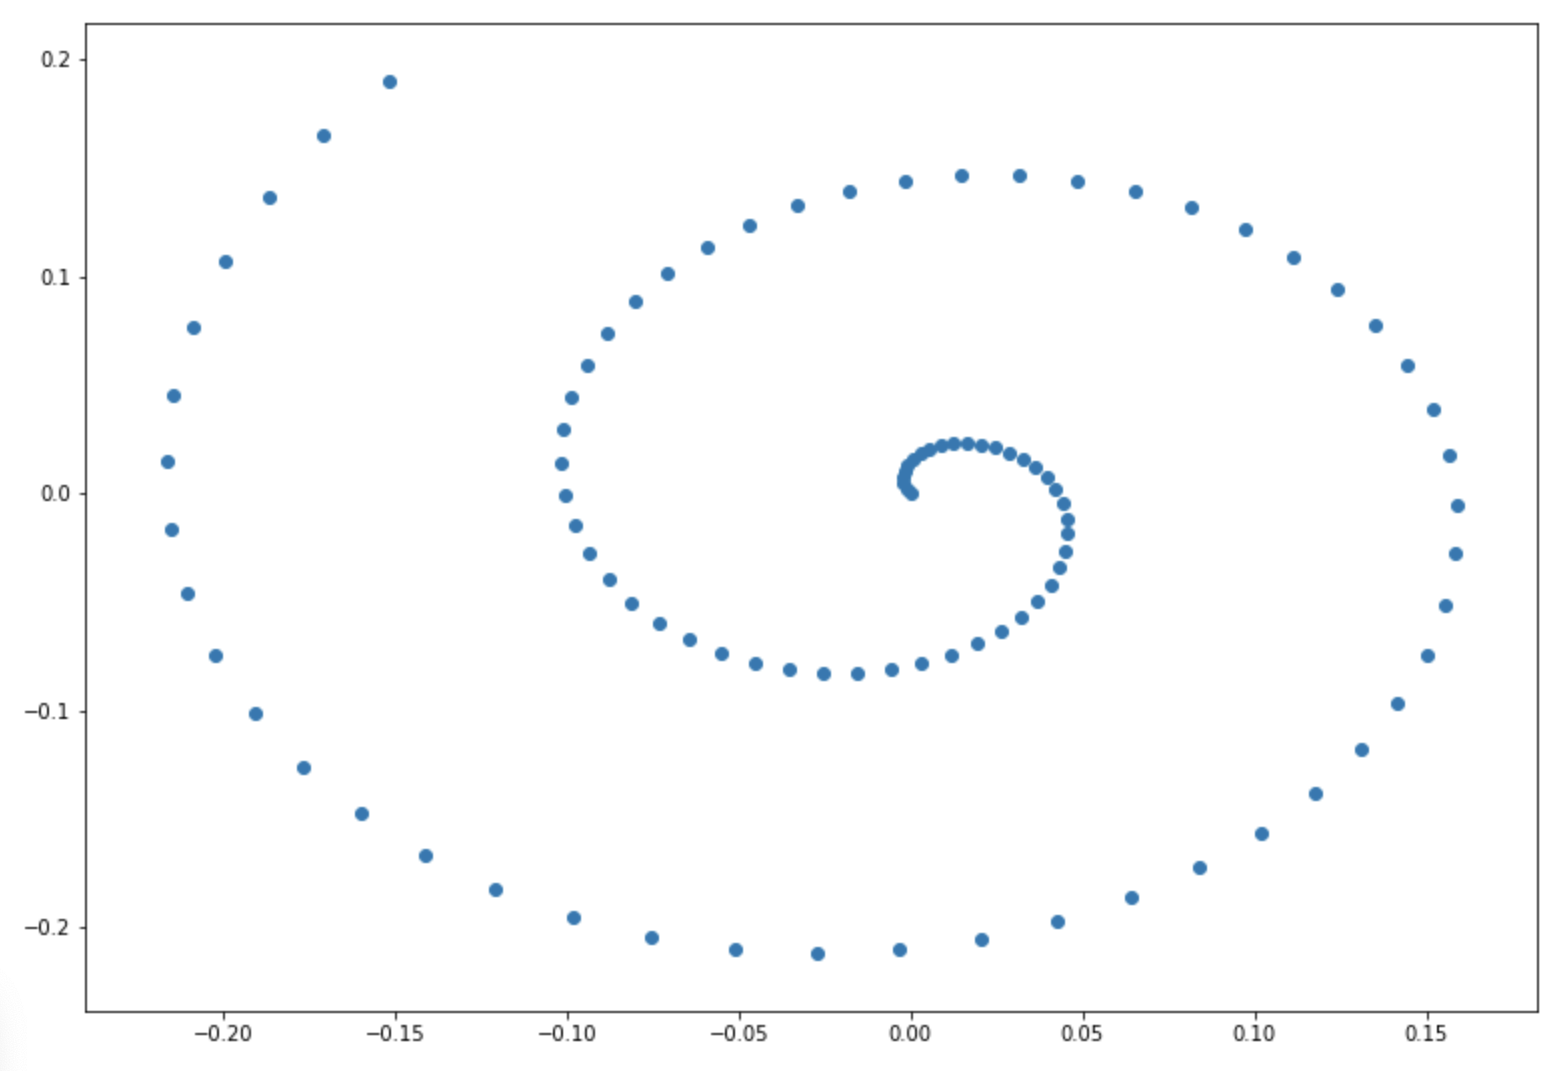
\includegraphics[width=70mm,scale=0.5]{images/q21.png}
      \label{fig:Q20_graph_1}
      \caption{}
  \end{figure}

  This behaviour is expected as the non-linear function is of the form $x_{i}sin(x_{i}), x_{i}cos(x_{i})$. It helps to view this with a parametric mindset. The parametric form of a circle is $sin(t),cos(t)$, but in our case we scale both parts by a monotonically increasing $t$ so the circle becomes a spiral. It is illustrative to view the points over a polar projection with a rough line at 0\textdegree \ as seen in Figure 12:
  
  \begin{figure}[H]
      \centering
      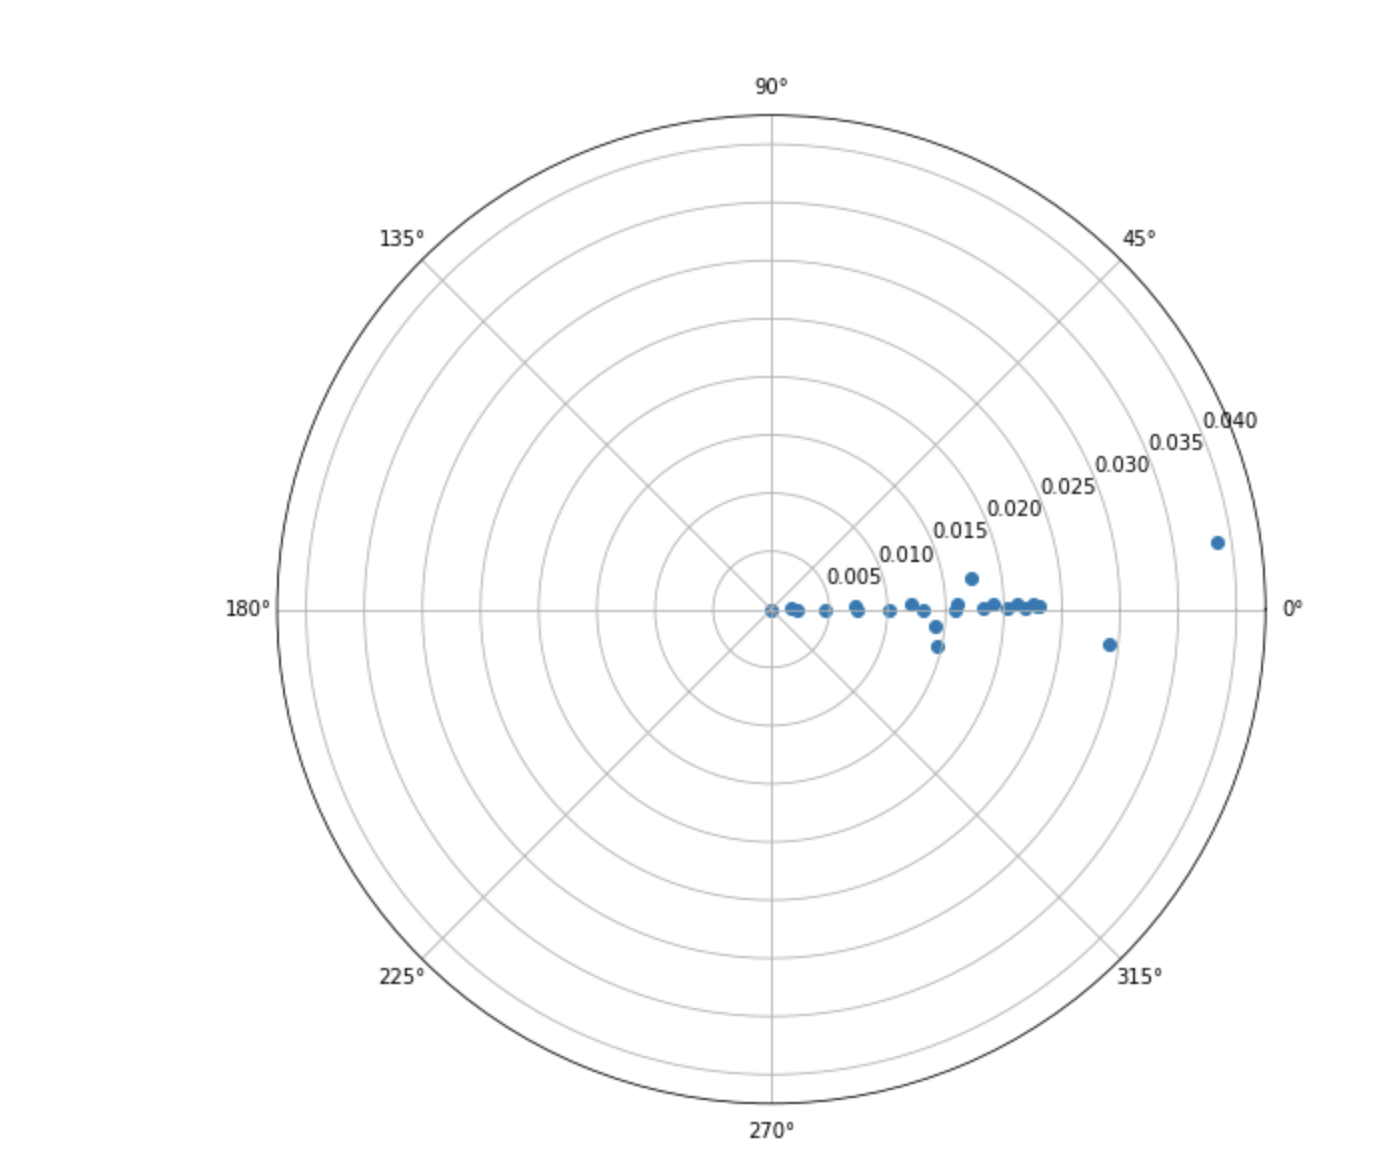
\includegraphics[width=70mm,scale=0.5]{images/q22polar.png}
      \label{fig:Q20_graph_1}
      \caption{}
  \end{figure}
  
  \textbf{Question 22}\\
  From Figure 13 we can see that there exists a direct mapping between the random subspace plot and the original plot. Although, the spiral has been rotated and scaled, the underlying shape has been preserved. This can be understood by analysing the formulation of the co-variance function.\\
  
  Let $\mathbf{R}$ be a rotation matrix
  \begin{align}
      \mathbf{C}(\mathbf{A'}) = \mathbf{C}(\mathbf{A}\mathbf{R}) &= \mathbf{A}\mathbf{R}(\mathbf{A}\mathbf{R})^T + \sigma^2\mathbf{I}\\
      &= \mathbf{A}\mathbf{R}\mathbf{R}^T\mathbf{A}^T + \sigma^2\mathbf{I}\\
      &= \mathbf{A}\mathbf{I}\mathbf{A}^T + \sigma^2\mathbf{I}\\
      &= \mathbf{A}\mathbf{A}^T + \sigma^2\mathbf{I}\\
      &= \mathbf{C}(\mathbf{A})
  \end{align}
  
  We see that the co-variance function is invariant to rotational transformation explaining why we have a rotated spiral compared to Figure 11.
  
 \begin{figure}[H]
      \centering
      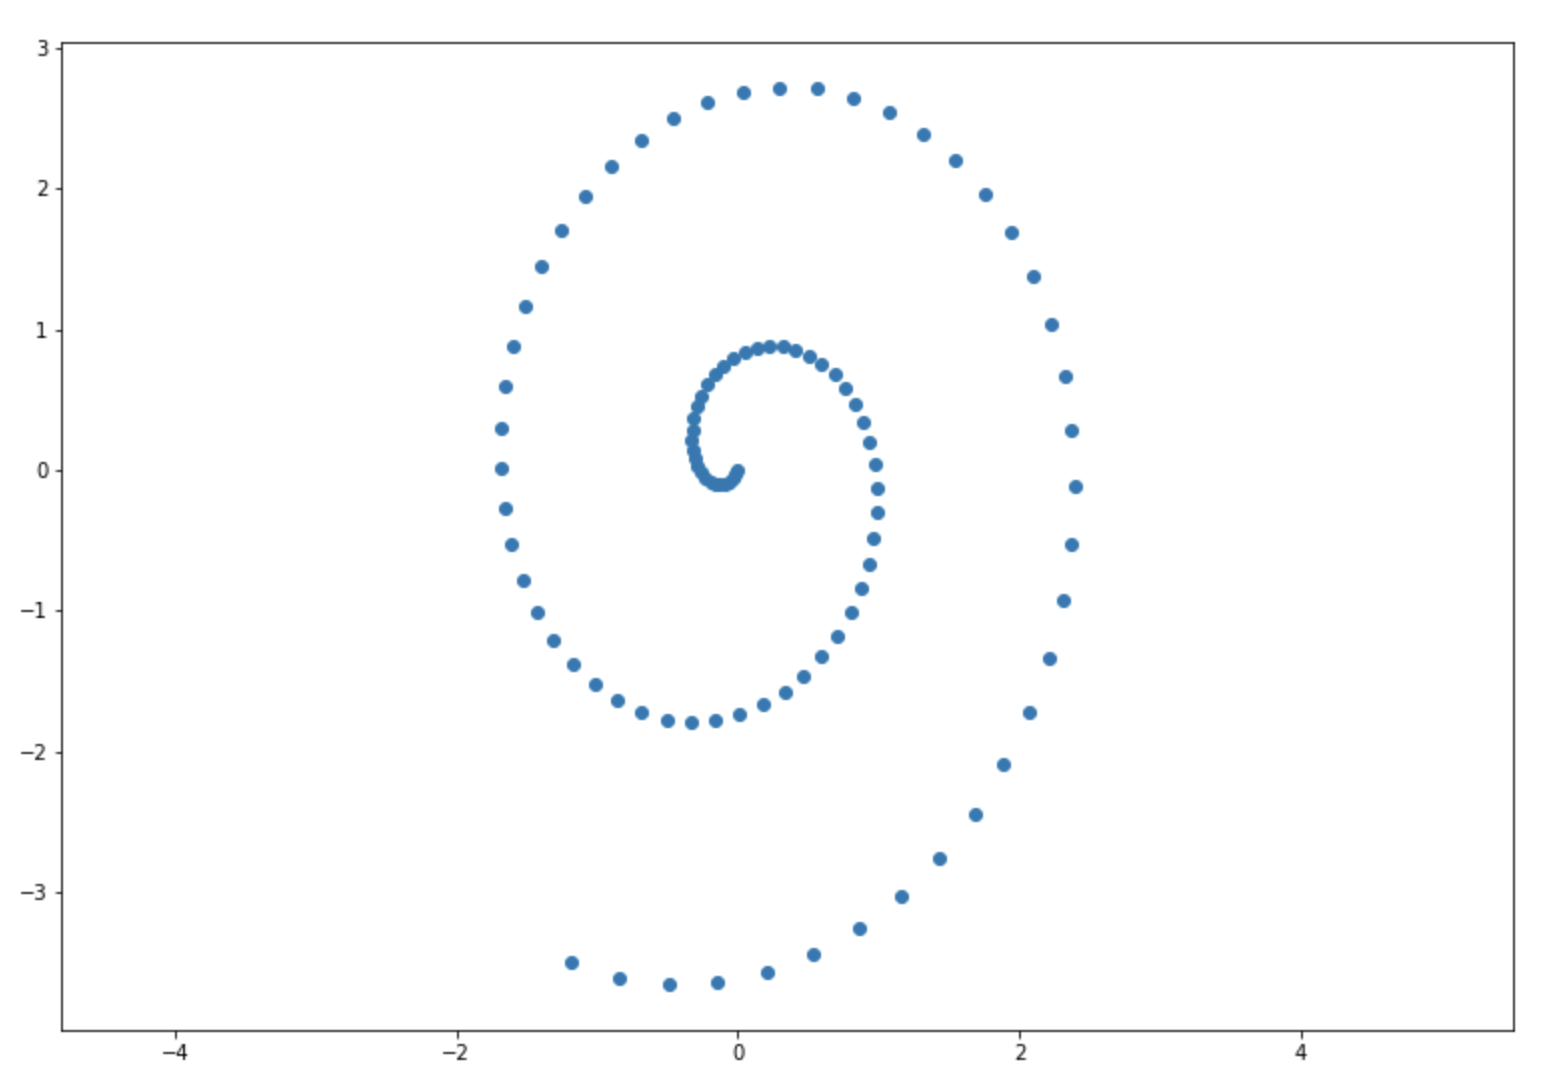
\includegraphics[width=70mm,scale=0.5]{images/Q22.png}
      \label{fig:Q20_graph_1}
      \caption{}
  \end{figure}
  
\section{Evidence}
  
  \textbf{Question 23}\\
  Before we can definitively determine the complexity of the given model, we must first define what we mean by 'complexity'. We can talk about algebraic complexity or we can talk about complexity with reference to flexibility and the size of the domain considered by the model.

  If we take parameter counting to be our metric of complexity, then we could view this as the simplest model, as it has no free parameters. The model simply defines a uniform distribution over the entire data set. This idea of measuring complexity by parameter counting is flawed, however. We could have instead made other models that only consider $10$ specific configurations, and then attributes to them a probability of $1/10$ and a probability of zero to all other configurations. This model would then have a higher evidence than other models that have many parameters. There exist other "zero-parameter" models that can assign the exact same probability distributions as models that have any number of parameters. In effect, parameter counting is not a good measure of model complexity.
  
  If parameter counting is flawed metric of complexity, then how exactly do we define complexity? From \cite{murray2005note}, "Simple models choose to concentrate their probability mass around a limited number of data sets. Complex models predict that data will be drawn from a large range of possibilities." By this definition, our model can be considered a complex model as its distribution covers the entire data domain. An intuitive explanation of this is that it has the ability to place a probability on configurations that exhibit varying behaviours. Taking this approach, the concept of model complexity is synonymous with model flexibility.
  
  \textbf{Question 24}\\

  In what way is M1 more or less flexible than M2?
  While M1 has more parameters than M0, the data domain over which M1 defines a probability mass is much smaller than that of M0. M0 places a probability over a wider range of configurations and can therefore be considered more flexible even though it is a zero parameter model. 
  
  How does this model spread its probability mass over D?
  M1 considers configurations that have the same no of $1$'s in each column as equivalent because the only information we have is about $x_1$ as it ignores the second dimension of $\mathbf{x}$. Therefore M1 gives high probability to each of these configurations and the probability mass over D is greater at these configurations. As every probability distribution integrates to $1$, the probability mass must be therefore be lower than M0 for some other configuration in our data domain. Furthermore, M1 is incapable of modelling certain configurations with horizontally oriented decision boundaries as it has no information about the 2nd dimension of $\mathbf{x}$ (only has one degree of freedom).
  
  How have the choices we've made restricted the distribution of the model?
  By choosing the number of parameters for each model, we have made some of these models (specifically M1 and M2) incapable of accounting for certain distributions. As a result of this we have restricted the distribution of the model as there are configurations to which some of our models give zero probability.
  
  In what way are the different models more flexible and in what way are they restrictive? Intuitively, we can view M0 as the most flexible model because its probability mass function covers the entire data domain and thus can model a greater range of configurations than the models with non-zero parameter count. In this regard, M1 and M2 are more restrictive because their probability mass function covers a smaller subset of the data domain. M3 is more flexible than both M1 and M2 as it covers a larger data domain. The models and their relative flexibilities can be seen in Figure 14 (b).
  
  \textbf{Question 25}\\
  When we marginalise out $\mathbf{\theta}$, the uncertainty present in our prior $p(\mathbf{\theta}\mid \mathcal{M}_i)$ is filtered through to our likelihood. Choosing our prior to be $\mathcal{N} \sim (\mathbf{0}, 10^3 \mathbf{I})$ with zero mean and a large variance implies that we are uncertain about the parameters of the model $M_i$. We have no beliefs about the parameters and so we don't want to encode any assumptions in our prior.
  
  How does this choice of prior affect the model?
  Specifying a prior with large variance allows us to model a wider range of  $\mathbf{\theta}$ values. This corresponds to sharper decision boundaries in our model. If, however, we choose a stronger prior with small co-variance then the model would behave more like a uniform distribution over all configurations.\cite{murray2005note} 
  
  \textbf{Question 26}\\
  Due to the random nature of the samples, it would seem sensible to take multiple values of the sums and take an average to see the true trend of the data.\\
  
  
  \begin{center}
    \begin{tabular}{ |c|c| } 
    \hline
    Model 0 & 1.0\\
    \hline
    Model 1 & 0.9999999999999978\\
    \hline
    Model 2 & 1.0000000000000014\\ 
    \hline
    Model 3 & 1.0000000000000008\\
    \hline
    \end{tabular}
  \end{center}

  
  The evidence is a probability distribution, and so the total sum over the entire data domain is $1$. The summation for each of our models approximates to $1$. Model 0 is exactly 1 as it is just summing over $\frac{1}{512}$ 512 times. All the other models are close to 1 but not exactly. These inaccuracies arise from the Monte Carlo approximation of the integral.\\
  \textbf{Question 27}
  
 \begin{figure}[H]%
    \centering
    \subfloat[All data sets]{{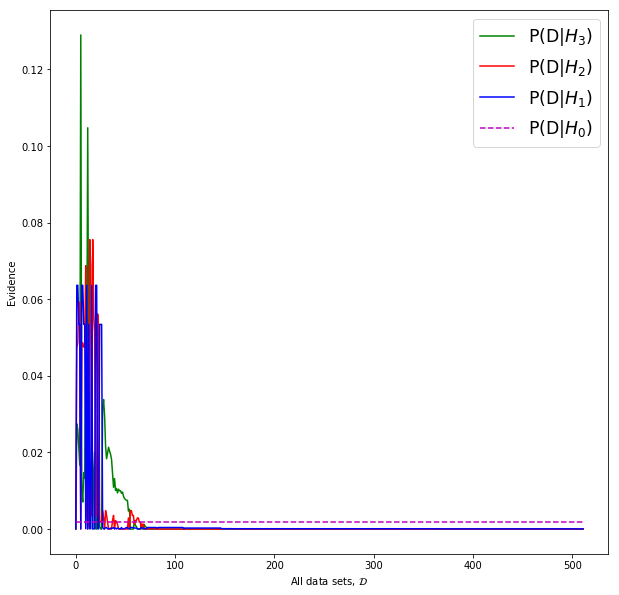
\includegraphics[width=7cm, scale =0.5]{imagesfinal/q27all.png}} }%
    \qquad
    \subfloat[Subset of data sets]{{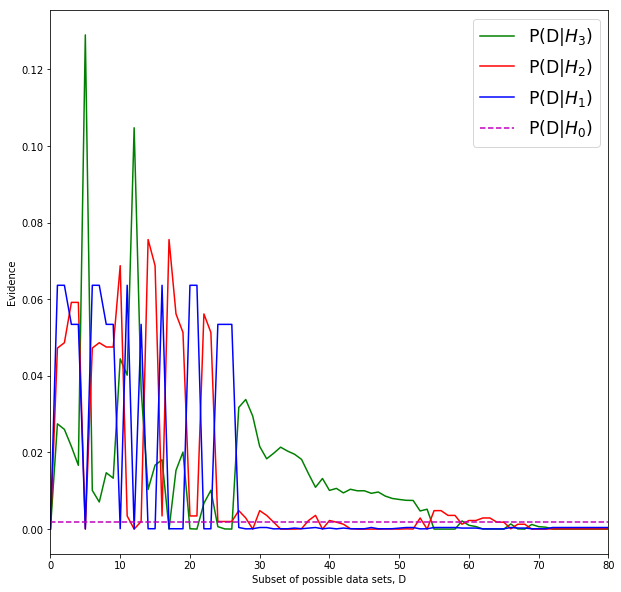
\includegraphics[width=7cm, scale =0.5]{imagesfinal/q27part.png}} }%
    \caption{Evidence against Data Set}%
    \label{fig:example}%
\end{figure}
  
  Looking at M1, M2 and M3:
  From the graphs we can see that models with a higher parameter count, cover more data . This more evident in Figure 11 (b) when we look at smaller a subset of dataset. Model 3, taking most parameters, cover the largest subset of the data space D. Due to the randomness of the samples, our graphs, although in agreement, are not exactly the same as the graphs in \cite{murray2005note}.\\\\
  
  \textbf{Question 28}\\
  
\begin{figure}[H]%
    \centering
    \subfloat[Min]{{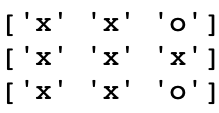
\includegraphics[width=2cm]{imagesfinal/min1.png}} }%
    \qquad
    \subfloat[Max]{{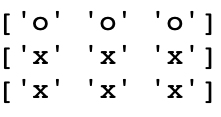
\includegraphics[width=2cm]{imagesfinal/max1.png}} }%
    \caption{Model 1}%
    \label{fig:example}%
\end{figure}
\begin{figure}[H]%
    \centering
    \subfloat[Min]{{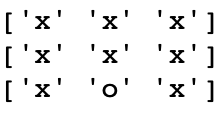
\includegraphics[width=2cm]{imagesfinal/min2.png}} }%
    \qquad
    \subfloat[Max]{{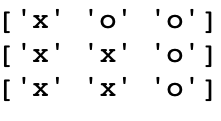
\includegraphics[width=2cm]{imagesfinal/max2.png}} }%
    \caption{Model 2}%
    \label{fig:example}%
\end{figure}
\begin{figure}[H]%
    \centering
    \subfloat[Min 3]{{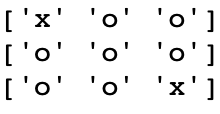
\includegraphics[width=2cm]{imagesfinal/min3.png}} }%
    \qquad
    \subfloat[Max 3]{{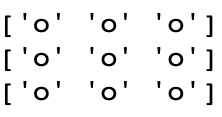
\includegraphics[width=2cm]{imagesfinal/max3.png}} }%
    \caption{Model 3}%
    \label{fig:example}%
\end{figure}

We can see that the most probable configuration for Model 3 is similar to the least probable configuration for Model 1 and 2. This is most likely due to Model 3 having a bias term which is capable of modelling unequal distributions of noughts and crosses (e.g all noughts). The omission of the bias term in Model 1 and 2, mean that is struggles with unequal distributions hence why our least probable elements look as they do.

Model 2 is unable to take into account the centre point, so ignoring that point our maximum should be a data set of equal distribution (4 crosses, 4 noughts) exactly as we see in Figure (16).

Model 1 is unable to take into account a whole axis. For the min for Model 1 we have that the far right axis has been ignored, so we have an uneven distribution of noughts to crosses hence why it gives the lowest probability. For the max, the bottom axis has been ignored, leaving it with an exactly equal number of noughts to crosses hence why gives it the highest probability.


  
  
  \textbf{Question 29}\\
  
  The parameters correspond to slope of the linear boundary. If the parameters ($\theta$) are large, we have a sharp decision boundary, but with small parameters ($\theta$) we will have a more gradual decision boundary.
  
  
   \begin{figure}[H]
      \centering
      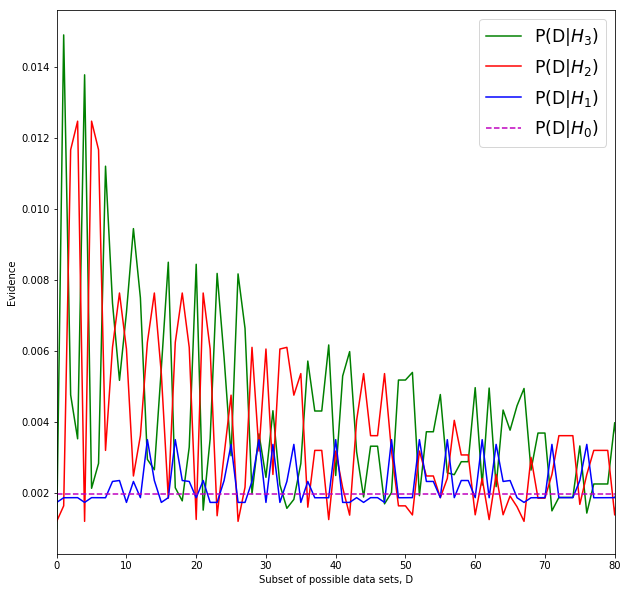
\includegraphics[width=50mm,scale=0.3]{imagesfinal/29partnond.png}
      \label{fig:example}
      \caption{Non-diagonal covariance}
  \end{figure}
  
  Using a co-variance matrix that is not diagonal implies that there is a correlation between the dimensions of the parameters ($\mathbf{\theta}$). This makes our evidence plot (Figure 18) vastly different to the original plot (Figure 14).
  
  
  \begin{figure}[H]
      \centering
      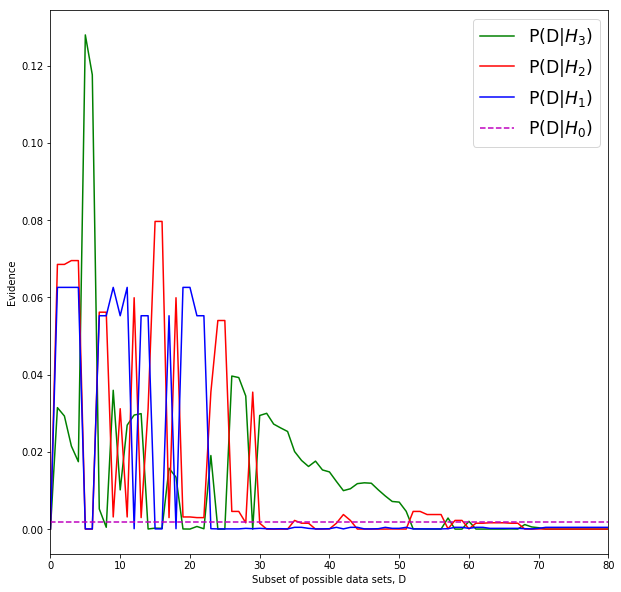
\includegraphics[width=50mm,scale=0.3]{imagesfinal/29mupart.png}
      \label{fig:example}
      \caption{$\mathbf{\mu} = [5, 5, 5]^T$}
  \end{figure}
  
  Changing the mean of the prior, produces a roughly similar evidence plot (Figure 19) when compared to the original (Figure 14). This is quite intuitive as we are assigning a very large variance over the distribution of the parameters ($\theta$),and so shifting the mean will have a little effect on each individual evidence value.
  
  \textbf{Question 30}\\ This coursework walked us through the most important concepts of machine learning. It created an intuition for the process by splitting it into easily understandable sections: prior, posterior and evidence. By the end of the coursework we appreciated the importance of each of these elements and how they come together to form coherent machine learning models. Outside of the strictly academic side of the course, we were also introduced to interesting concepts such as model complexity which piqued our curiosity for this area of mathematics and computer science. More importantly it taught us to abstract away from the lower level details and think about the philosophical aspect of this course of which we were previously unaware.  
  
\end{enumerate}

%----------------------------------------------------------------------------------------
%	BIBLIOGRAPHY
%----------------------------------------------------------------------------------------

%\printbibliography[title={Bibliography}] % Print the bibliography, section title in curly brackets

\bibliography{MLModels}{}
\bibliographystyle{abbrv}
\nocite{*}


%----------------------------------------------------------------------------------------

\end{document}